%% LaTeX Beamer presentation template (requires beamer package)
%% see http://bitbucket.org/rivanvx/beamer/wiki/Home
%% idea contributed by H. Turgut Uyar
%% template based on a template by Till Tantau
%% this template is still evolving - it might differ in future releases!

\documentclass[10pt]{beamer}

\mode<presentation>
{
\usetheme{Malmoe}

\setbeamercovered{transparent}
}


\addtobeamertemplate{navigation symbols}{}{%
\usebeamerfont{footline}%
\usebeamercolor[fg]{footline}%
\hspace{1em}%
\insertframenumber/\inserttotalframenumber
}

\useoutertheme{infolines}
\setbeamertemplate{footline}{} 

\usepackage[brazil]{babel}
\usepackage[utf8]{inputenc}
\usepackage{listings}

% font definitions, try \usepackage{ae} instead of the following
% three lines if you don't like this look
\usepackage{mathptmx}
\usepackage[scaled=.90]{helvet}
\usepackage{courier}
\usepackage{url}


\usepackage[T1]{fontenc}

\title{Reprodução de um elemento do artigo \textit{Accelerating Decoupled
Look-ahead via Weak Dependence Removal: A Metaheuristic Approach}}

%\subtitle{}

% - Use the \inst{?} command only if the authors have different
%   affiliation.
%\author{F.~Author\inst{1} \and S.~Another\inst{2}}
\author{Gustavo Ciotto Pinton}

% - Use the \inst command only if there are several affiliations.
% - Keep it simple, no one is interested in your street address.
\institute
{

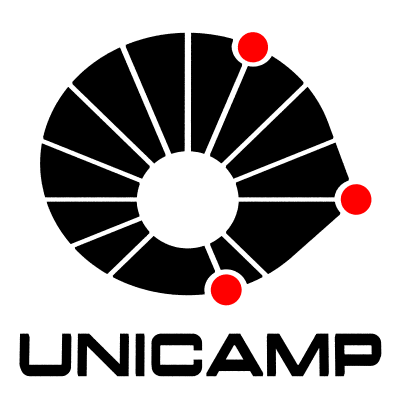
\includegraphics[scale=0.12]{logo} \\
\vspace{16pt}
Universidade Estadual de Campinas - UNICAMP\\
MO601B - Arquitetura de Computadores}

\date{18 de Novembro de 2016}



% If you have a file called "university-logo-filename.xxx", where xxx
% is a graphic format that can be processed by latex or pdflatex,
% resp., then you can add a logo as follows:

% \pgfdeclareimage[height=0.5cm]{university-logo}{university-logo-filename}
% \logo{\pgfuseimage{university-logo}}



% Delete this, if you do not want the table of contents to pop up at
% the beginning of each subsection:
\AtBeginSubsection[]
{
\begin{frame}<beamer>
\frametitle{Outline}
\tableofcontents[currentsection,currentsubsection]
\end{frame}
}

% If you wish to uncover everything in a step-wise fashion, uncomment
% the following command:

%\beamerdefaultoverlayspecification{<+->}

\begin{document}

\begin{frame}

\titlepage
\end{frame}

\begin{frame}
\frametitle{Sumário}
\tableofcontents
\end{frame}

\section{Motivação}


\begin{frame}
\frametitle{Motivação}
\begin{itemize}
\item Apesar da proliferação de sistemas \textit{multi-core} e
\textit{multi-threaded}, a performance de aplicações \textit{single-thread}
ainda é um objetivo importante.

\item Aplicações \textit{single-threaded} fazem uso do paralelismo de
instruções.

\item Desafios: como explorar este paralelismo sem muitos custos adicionais

\item Alternativa: \textit{Decoupled look-ahead architecture} 
\end{itemize}

\centering
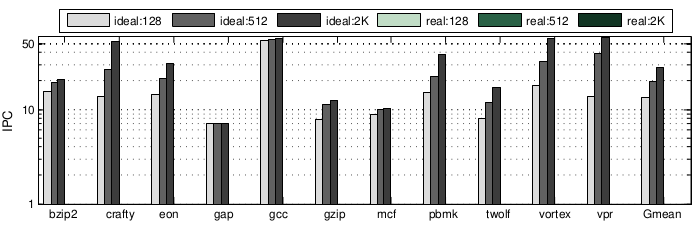
\includegraphics[width=0.9\textwidth]{images/single-ipc}

\end{frame}

\begin{frame}
\frametitle{Contagem de acessos à memória}
\framesubtitle{Páginas de 4KB}



\end{frame}

\begin{frame}
\frametitle{Contagem de acessos à memória}
\framesubtitle{Páginas de 4MB}




\end{frame}

\begin{frame}
\frametitle{Contagem de acessos à memória}
\framesubtitle{\textit{Toy benchmark}}

\begin{itemize}
\begin{itemize}

\end{itemize}

\end{itemize}

\end{frame}

\begin{frame}
\frametitle{Contagem de acessos à memória}
\framesubtitle{\textit{Toy benchmark}}

 
\end{frame}

\begin{frame}
\frametitle{Conclusões}
\framesubtitle{Resultados}

\begin{itemize}

\end{itemize}

\end{frame}


\begin{frame}
\frametitle{Referências}

\begin{itemize}
  \item Henning, J. L. (2007). Spec cpu2006 memory footprint. \textit{ACM
  SIGARCH Computer Architecture News}, 35;
  \vspace{14pt}
  \item SniperSim (2008). Pinballs, disponível em
  \url{http://snipersim.org/w/Pinballs}.
  \item Intel® 64 and IA-32 Architectures
Software Developer’s Manual, disponível em \url{http://intel.ly/KqEL7c}.
\end{itemize}

\end{frame}

\end{document}
